\subsection{Matrix element method}
\label{subsec:MEM}
The matrix element method~\cite{kondo1} links directly
theoretical calculations and observed quantities,  making the most complete 
use of the kinematic information in an event. 
%has been used by the D0 and CDF 
%collaborations for precision measurements of the top quark 
%mass~\cite{d0_topmass,cdf_topmass} and for the observations of single top 
%quark production~\cite{d0_stop,cdf_stop}. Recently this technique has 
%been used for the \tth\ search by the
%CMS experiment~\cite{CMSMEM}. 

Given an observation, defined by the four-momentum vectors of all final-state objects at reconstruction level, $\MB{x}$,
the method calculates the probability 
of the event to be consistent with physics process $i$ 
described by a set of parameters $\MB{\alpha}$. 
This probability density function $P_i \left ( \MB{x} | \MB{\alpha} \right )$
is defined as:

\begin{equation}
P_i\left(\MB{x}|\MB{\alpha}\right) = \frac{(2\pi)^4}{\sigma_i^{\mathrm{exp}}\left(\MB{\alpha}\right)} 
\int \dif{\SUB{p}{a}} \dif{\SUB{p}{b}} \; f(\SUB{p}{a}) f(\SUB{p}{b}) \;
 \frac{\left|\mathcal{M}_{i}\left(\MB{y}|\MB{\alpha}\right)\right|^2}{\mathcal{F}} \;
W\left(\MB{y}|\MB{x}\right) \; \dif{\Phi_N}\left(\MB{y}\right)~,
\end{equation}

\noindent and is obtained by numerical integration
over the entire phase space of the initial- and final-state particles. 
The transfer functions $W\left(\MB{y}|\MB{x}\right)$ map the detector quantities
$\MB{x}$ to the parton level quantities $\MB{y}$.
The transition matrix 
element $\mathcal{M}_{i}\left(\MB{y}|\MB{\alpha}\right)$ is defined by the Feynman diagrams of the hard process considered, $i$. 
The flux factor $\mathcal{F}$ and the Lorentz-invariant phase space element 
$\dif{\Phi_N}$ describe the kinematics of the process, and $f\left(\SUB{p}{a,b}\right)$ are parton distribution functions.  
Finally, the \xsec\ 
$\sigma_i^{\mathrm{exp}}$ normalizes $P_i$ to unity 
taking acceptance and efficiency into account.

The assignment of reconstructed objects to final-state partons in the hard process 
contains multiple ambiguities. The process probability is computed for each allowed assignment permutation 
of the jets to the final-state quarks of the hard process.
A process likelihood function can then be built 
by summing the process probabilities for the $N_{p}$ allowed assignment 
permutations:

\begin{equation}
\mathcal{L}_{i}  \left (\MB{x}|\MB{\alpha}\right )  = \sum_{p=1}^{N_{p}} \strut P_{i}^{p}
\left (\MB{x}|\MB{\alpha} \right ). 
\label{eq:SSLL}
\end{equation}

The process probability densities are used to distinguish signal from 
background events by calculating the likelihood ratio of the signal and 
background processes contributing with fractions $f_{\textrm{bkg}}$,

\begin{equation}
r_{\textrm{sig}} \left  ( \MB{x} | \MB{\alpha} \right ) = 
\frac{\mathcal{L}_{\textrm{sig}} \left (\MB{x}|\MB{\alpha} \right )}
{\sum\limits_{\textrm{bkg}} f_{\textrm{bkg}} \mathcal{L}_{\textrm{bkg}} 
\left (\MB{x}|\MB{\alpha} \right ) } \label{eq:neyman}~. 
\end{equation} 

This ratio, according to the Neyman--Pearson lemma~\cite{neymanpearson}, is the 
most powerful discriminant between signal and background processes. In the analysis, 
this variable is used as input to the NN along with other kinematic variables. 
 
The integration is performed with \textsc{VEGAS}~\cite{VEGAS} using adaptive MC techniques~\cite{gsl}.
Matrix element calculations are generated with \madgraphfive\ at LO. 
The transfer functions are obtained from simulation~\cite{klfitter} and the parton
distribution functions are taken from the {\sc CTEQ6L1} set from the \textsc{LHAPDF} package~\cite{lhapdf}.

%The integration is performed using \textsc{VEGAS}~\cite{VEGAS}.  Due to the complexity and 
%high dimensionality, adaptive MC techniques~\cite{gsl}, 
%simplifications and approximations are needed to obtain results 
%within a reasonable computing time.
%In particular, only the numerically most significant contributing helicity states of a 
%process hypothesis for a given event,  
%identified at the start of each integration, are evaluated. This does not 
%perceptibly decrease the separation power but reduces the calculation time by 
%more than an order of magnitude. 
%Furthermore, several approximations are made to improve the {\sc VEGAS} convergence rate. 
%Firstly, the dimensionality of integration is reduced by assuming that the final-state object 
%directions in \eta{} and $\phi$ as well as charged lepton momenta are well measured, and therefore 
%the corresponding transfer functions are represented by $\delta$ functions. 
%The total momentum conservation and a negligible transverse momentum of the 
%initial-state partons allow for further reduction.
%Secondly, kinematic transformations are utilised to optimise the integration over the remaining 
%phase space by aligning the peaks of the integrand with the integration dimensions. 
%The narrow-width approximation is applied to the leptonically decaying $W$ boson. 
%This leaves three $b$-quark energies, one light-quark energy, the hadronically decaying 
%$W$ boson mass and the invariant mass of the two $b$-quarks
%originating from either the Higgs boson for the signal  
%or a gluon for the background as the remaining parameters which define the integration phase space.
%The total integration volume is restricted based  upon the observed values and the width 
%of the transfer functions and of the 
%propagator peaks in the matrix elements. Finally, the likelihood 
%contributions of all allowed assignment permutations are coarsely integrated, and  
%only for the leading twelve assignment permutations is the full integration performed, 
%with a required precision decreasing according to their relative contributions.

\begin{figure}[tb!]
\begin{center}
  \begin{subfigure}{0.49\textwidth}

\includegraphics[width=\textwidth]{Analysis/Figures_ttH/ttHbb_fusion.png}
\caption{}\label{fig:feyn_ttH_1} \end{subfigure}
%\begin{subfigure}{0.49\textwidth} %Change caption
%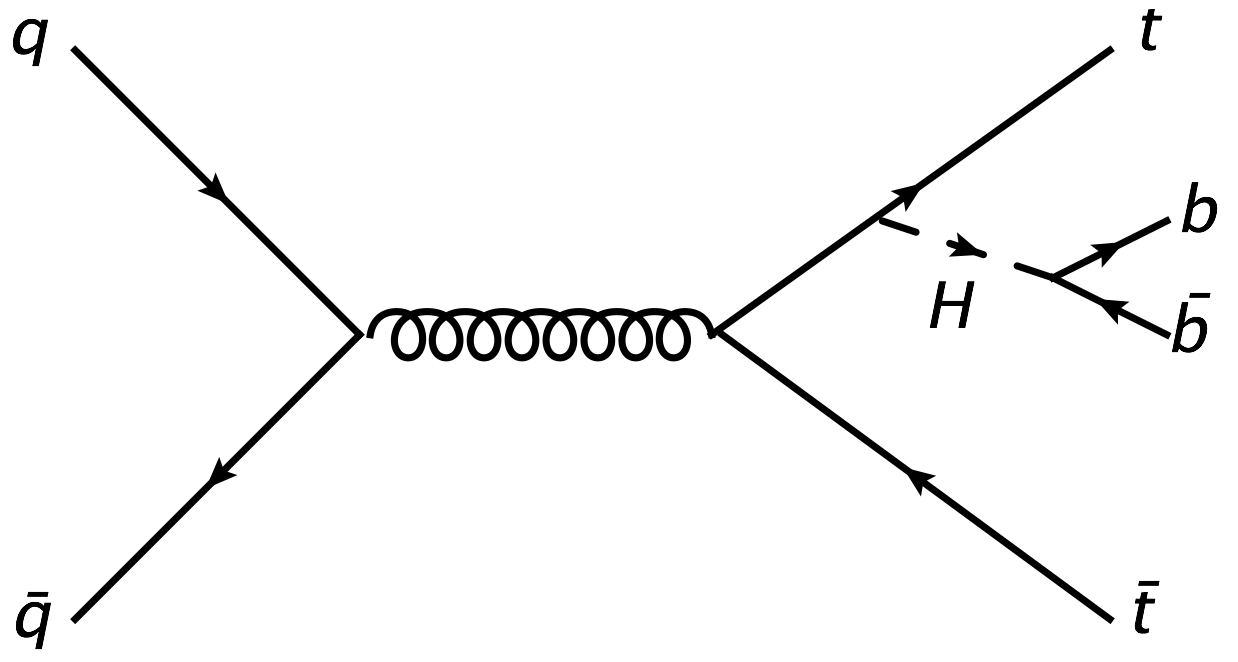
\includegraphics[width=\textwidth]{Analysis/Figures_ttH/ttHbb_radiation.png} 
%\caption{}\label{fig:feyn_ttH_2} \end{subfigure}
\begin{subfigure}{0.49\textwidth}
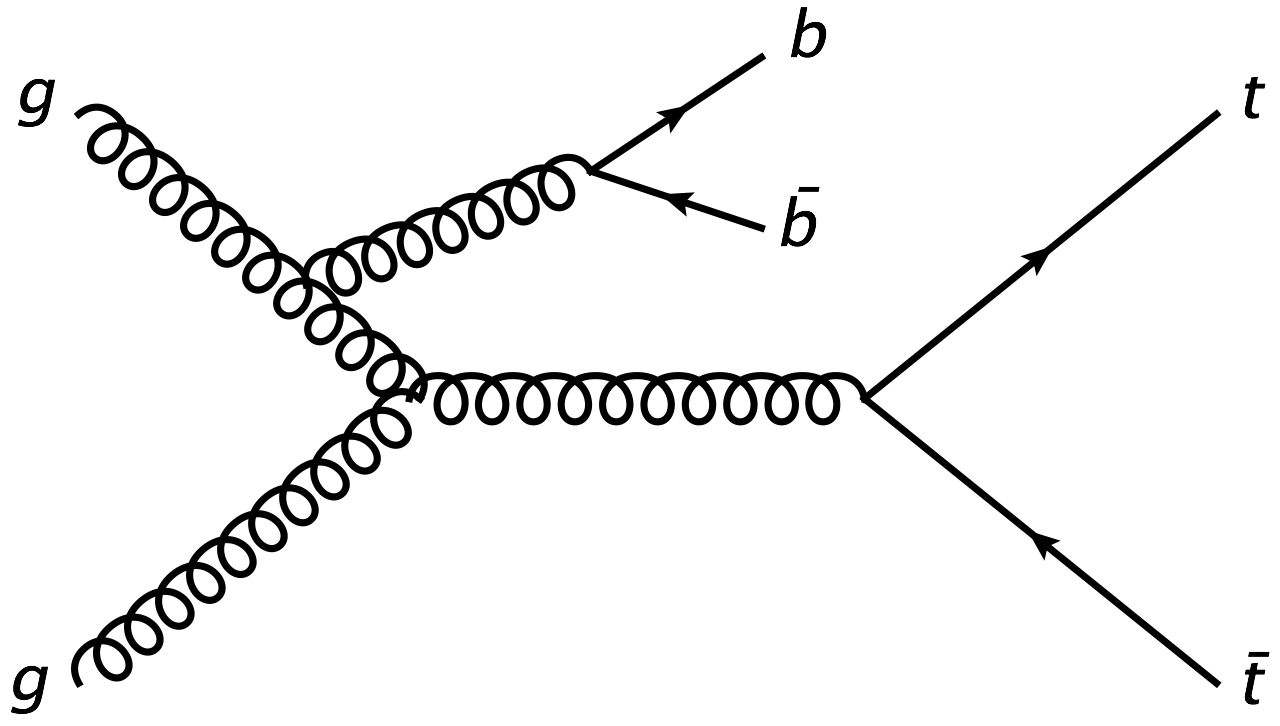
\includegraphics[width=\textwidth]{Analysis/Figures_ttH/ttbb.png}
\caption{}\label{fig:feyn_ttbb} \end{subfigure}
\caption{(a) Representative tree-level Feynman diagrams for the production of the Higgs boson in association with a top pair (\tth) and the subsequent decay of the Higgs to \bbbar, (b) and for the main background \ttbar+\bbbar. 
}
\label{fig:feynman}
\end{center}
\end{figure}

The signal hypothesis is defined as a SM Higgs boson produced in association
with a top-quark pair as shown in figure~\ref{fig:feyn_ttH_1}. 
The Higgs boson is required to decay into \bbbar, while the top-quark pair decays 
into the single-lepton channel. 
For the background hypothesis, only the diagrams of the irreducible 
\ttbb\ background are considered, as shown in figure~\ref{fig:feyn_ttbb}. Since it dominates the most signal-rich analysis regions, 
the inclusion of other processes does not improve the separation 
between signal and background. 
%No gluon radiation from the 
%final-state quarks is  
%allowed, since these are kinematically suppressed and difficult to treat in any kinematic 
%transformation aiming for phase-space alignment during the integration process.
%In the definition of the signal and background hypothesis the LO diagrams are 
%required to have a top-quark pair as an intermediate state resulting in exactly 
%four $b$-quarks, two light quarks, one charged lepton (electron or muon) and one neutrino 
%in the final state. Assuming lepton universality and invariance under charge 
%conjugation,  
%diagrams of only one lepton flavour and of only negative charge (electron) are considered.
The probability density function calculation of the signal and background is only performed in the \sixthree\ 
and \sixfour\ regions. 

Only six reconstructed 
jets are considered in the calculation: 
the four jets with the highest value of the probability to be a $b$-jet returned by the 
$b$-tagging algorithm (i.e. the highest $b$-tagging weight) 
and two of the remaining jets with an 
invariant mass closest to the $W$ boson mass of 80.4 \gev. 
%If a jet is $b$-tagged it cannot be 
%assigned to a light quark in the matrix element description. In the case of more than four 
%$b$-tagged jets, only the four with the highest $b$-tagging weight are treated as $b$-tagged. 
Assignment permutations between the two light quarks of the hadronically decaying $W$ 
boson and between 
the two $b$-quarks originating from the Higgs boson or gluon result in the same 
likelihood value and are thus not considered.
As a result there are in total 12 and 36 assignment permutations in the \sixfour\ 
and \sixthree\ regions, respectively, which need to be integrated.

Using the \tth\ process as the signal hypothesis and the \ttbb\ process as the 
background hypothesis, a slightly modified version of equation~(\ref{eq:neyman}) is used to define 
the likelihood ratio $D1$:

\begin{equation}
 D1=\frac{\mathcal{L}_{t\bar{t}H}}{{\mathcal{L}_{t\bar{t}H}} + 
 \alpha \cdot \mathcal{L}_{t\bar{t}+b\bar{b}}}\
\label{eq:ME_D1} ,
\end{equation}

\noindent where $\alpha=0.23$ is a relative normalization factor chosen to optimize the
performance of the discriminant given the finite bin sizes of the $D1$ distribution. 
In this definition, 
signal-like and background-like events have $D1$ values close to one and zero, 
respectively.   
The logarithm of the summed signal likelihoods defined by equation~(\ref{eq:SSLL}) 
and the ratio $D1$ are included in the 
NN training in both the \sixthree\ and \sixfour\ regions. 

The $D1$ variable provides the best separation between the
\tth\ signal and the dominant \ttbb\ background in the \sixfour\ region, and the 
SSLL variable introduces further separation to the rest of the backgrounds.  
Figure~\ref{fig:MEM_separation} shows the discrimination power of the $D1$ and SSLL variables in the \sixthree\ and \sixfour\ regions.
\begin{figure}[tb!]
  \centering
  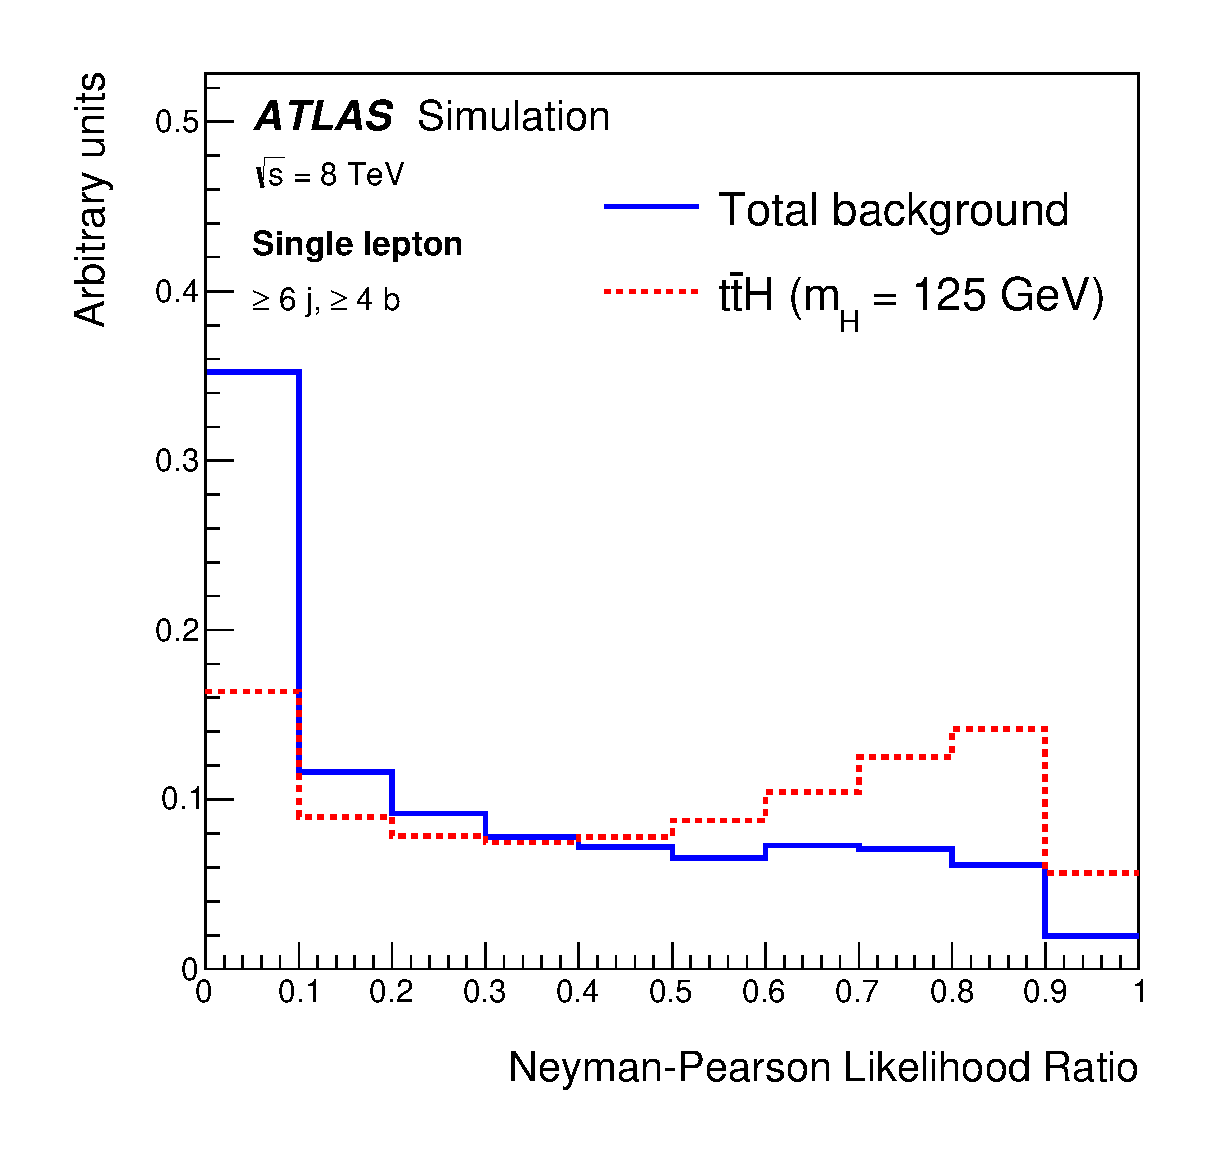
\includegraphics[width=0.49\textwidth]{Analysis/Figures_ttH/ME_D1_6jincl_sep.eps}
  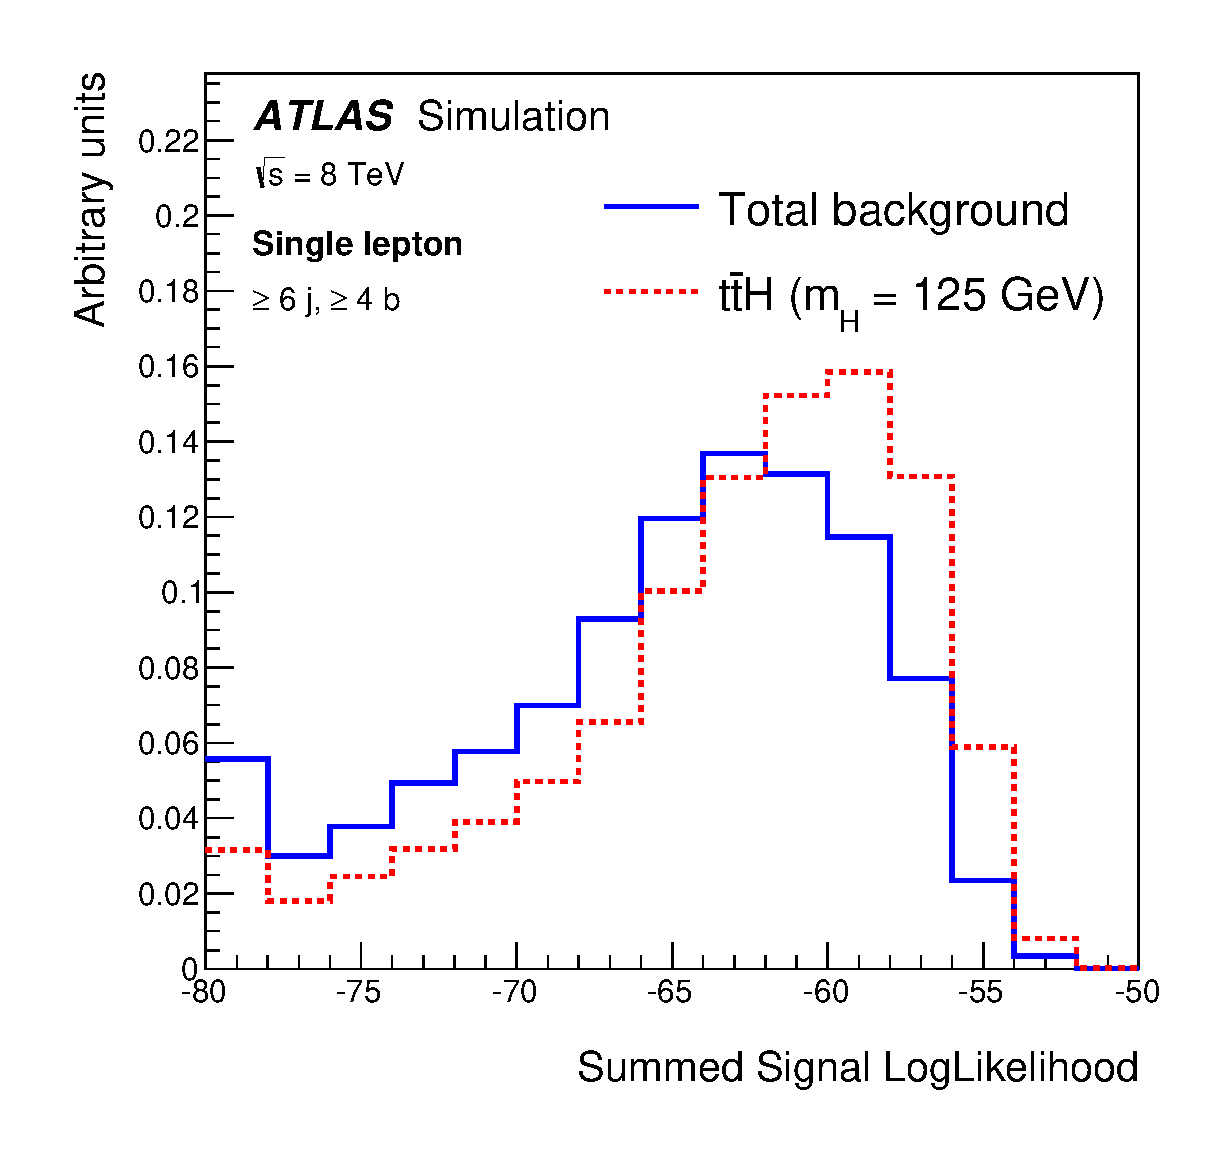
\includegraphics[width=0.49\textwidth]{Analysis/Figures_ttH/ME_SLL_6jincl_sep.eps}
  \caption{Expected distributions for $D1$ and SSLL in the \tth\ signal and total background in the \sixfour\ region.}
  \label{fig:MEM_separation}
\end{figure}

